\documentclass[]{beamer}
% Class options include: notes, notesonly, handout, trans,
%                        hidesubsections, shadesubsections,
%                        inrow, blue, red, grey, brown

% Theme for beamer presentation.
\usepackage{beamerthemesplit} 
% Other themes include: beamerthemebars, beamerthemelined, 
%                       beamerthemetree, beamerthemetreebars  

\title{PHY115}    % Enter your title between curly braces
\author{Motion in More Than one Dimension}                 % Enter your name between curly braces
\institute{Digipen}      % Enter your institute name between curly braces
\date{Spring 2023} 

\begin{document}

% Creates title page of slide show using above information
\begin{frame}
  \titlepage
\end{frame}
%\note{Talk for 30 minutes} % Add notes to yourself that will be displayed when
                           % typeset with the notes or notesonly class options

\section[]{}

% Creates table of contents slide incorporating
% all \section and \subsection commands
\begin{frame}
  \tableofcontents
\end{frame}


%%%%%%%%%%%%%%%%%%%%%%%%%%%%%%%%%%%%%%%%%%%%%%%%%%%%%%%%%%%%%%%%%%%

\section{Motion in two or three dimensions}
%%%%%%%%%%%%%%%%%%%%%%%%%%%%%%%%%%%%%%%%%%%%%%%%%%%%%%%%%%%%%%%%%%%

\begin{frame}
    Position and velocity Vectors
    \vspace{3mm}
 
    \begin{columns}[c]
        \column{2in}  % slides are 3in high by 5in wide
       
        \begin{equation}
          \vec{r}=x\hat{\imath}+y\hat{\jmath}+z\hat{k}
         \end{equation}
      
  
    
        \column{2.5in}
        
        \begin{figure}[h!]  
       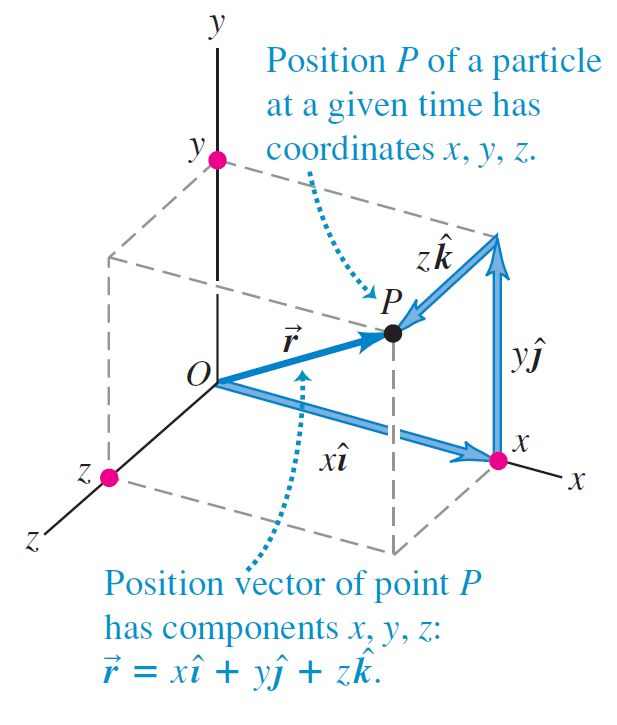
\includegraphics[width=0.8\textwidth]{images/7.jpg}
        \caption{ {\tiny Figure from Sears and Zemansky's University Physics 
        with Modern Physics, 13th Edition.} }
     \end{figure}
     
     
     
        \end{columns}
    
\end{frame}


%%%%%%%%%%%%%%%%%%%%%%%%%%%%%%%%%%%%%%%%%%%%%%%%%%%%%%%%%%%%%%%%%%%

\begin{frame}
    Position and velocity Vectors
    \vspace{3mm}
 
    \begin{columns}[c]
        \column{2in}  % slides are 3in high by 5in wide
       
        \begin{equation}
          \vec{r}=x\hat{\imath}+y\hat{\jmath}+z\hat{k}
         \end{equation}
         \vspace{3mm}
      

        \begin{equation}
            \vec{v}_{av}=\frac{\vec{r}_2-\vec{r}_1}{t_2-t_1}=\frac{\Delta \vec{r}}{\Delta{t}}
        \end{equation}
     
        \vspace{3mm}
     
        
    
        \column{2.5in}
        
        \begin{figure}[h!]  
       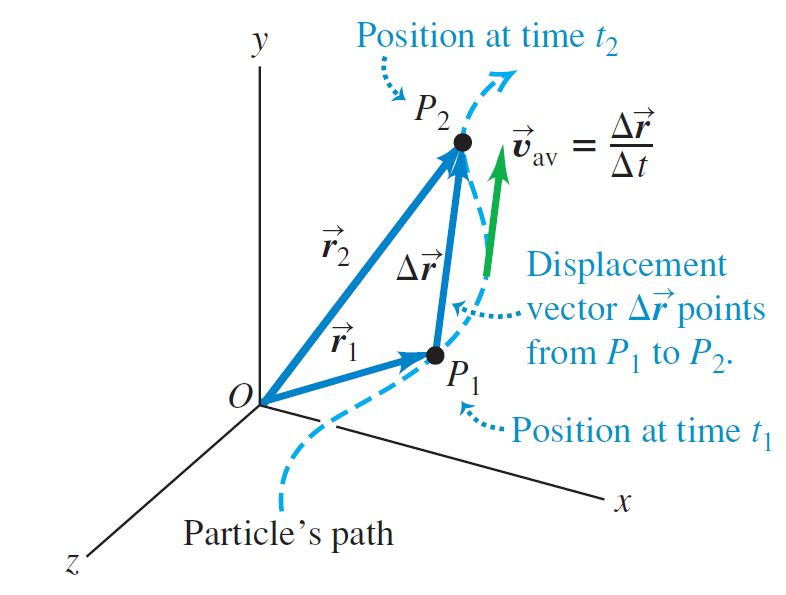
\includegraphics[width=1.\textwidth]{images/8.jpg}
        \caption{ {\tiny Figure from Sears and Zemansky's University Physics 
        with Modern Physics, 13th Edition.} }
     \end{figure}
     
     
     
        \end{columns}
    
\end{frame}

%%%%%%%%%%%%%%%%%%%%%%%%%%%%%%%%%%%%%%%%%%%%%%%%%%%%%%%%%%%%%%%%%%%

\begin{frame}
    Position and velocity Vectors
    \vspace{3mm}
 
    \begin{columns}[c]
        \column{2in}  % slides are 3in high by 5in wide
       
        \begin{equation}
          \vec{r}=x\hat{\imath}+y\hat{\jmath}+z\hat{k}
         \end{equation}
         \vspace{3mm}
      

        \begin{equation}
            \vec{v}_{av}=\frac{\vec{r}_2-\vec{r}_1}{t_2-t_1}=\frac{\Delta \vec{r}}{\Delta{t}}
        \end{equation}
     
        \vspace{3mm}
     
        
       \begin{equation}
           \vec{v}=\lim_{\Delta t\to 0}\frac{\vec{r}_2-\vec{r}_1}{t_2-t_1}=\frac{\Delta \vec{r}}{\Delta{t}}
       \end{equation}
    
        \column{2.5in}
        
        \begin{figure}[h!]  
       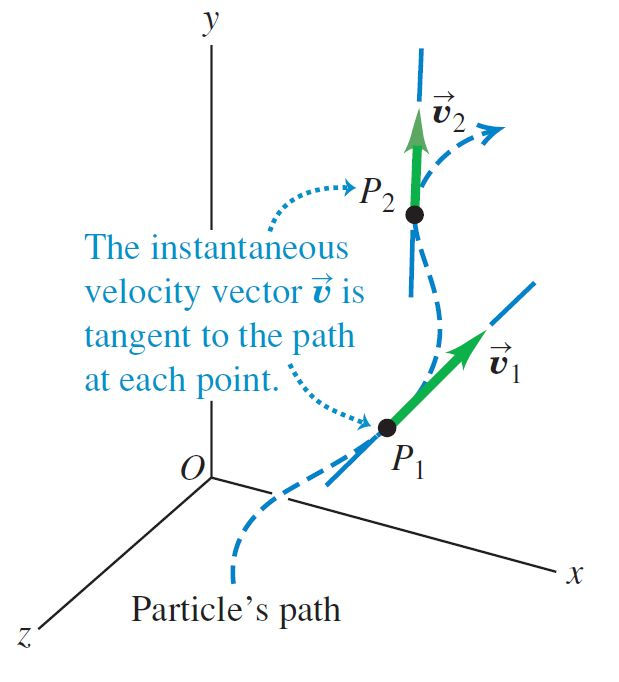
\includegraphics[width=0.8\textwidth]{images/9.jpg}
        \caption{ {\tiny Figure from Sears and Zemansky's University Physics 
        with Modern Physics, 13th Edition.} }
     \end{figure}
     
     
     
        \end{columns}
    
\end{frame}



%%%%%%%%%%%%%%%%%%%%%%%%%%%%%%%%%%%%%%%%%%%%%%%%%%%%%%%%%%%%%%%%%%%

\begin{frame}
The Instantaneous velocity is,

    \vspace{3mm}

         \begin{equation}
          \vec{v}=\frac{dx}{dt}\hat{\imath}+\frac{dy}{dt}\hat{\jmath}+\frac{dz}{dt}\hat{k}
         \end{equation}
   \vspace{3mm}
where,

   \begin{equation}
        v_x=\frac{dx}{dt},~ v_y=\frac{dy}{dt}~and~v_z=\frac{dz}{dt}
         \end{equation}

        \vspace{3mm}
Its magnitude is,


        \vspace{3mm}



         \begin{equation}
          |\vec{v}|=\sqrt{v^2_x+v^2_y+v^2_z}
         \end{equation}



\end{frame}


%%%%%%%%%%%%%%%%%%%%%%%%%%%%%%%%%%%%%%%%%%%%%%%%%%%%%%%%%%%%%%%%%%%

\begin{frame}
When the motion is in the $x-y$-plane

    \vspace{3mm}



 
    \begin{columns}[c]
        \column{2in}  % slides are 3in high by 5in wide
       




         \begin{equation}
          \vec{v}=\frac{dx}{dt}\hat{\imath}+\frac{dy}{dt}\hat{\jmath}
         \end{equation}



        \vspace{3mm}



         \begin{equation}
          |\vec{v}|=\sqrt{v^2_x+v^2_y}
         \end{equation}



        \vspace{3mm}

         \begin{equation}
        tan \alpha=\frac{v_y}{v_x}
         \end{equation}



        \column{2.5in}
        
        \begin{figure}[h!]  
       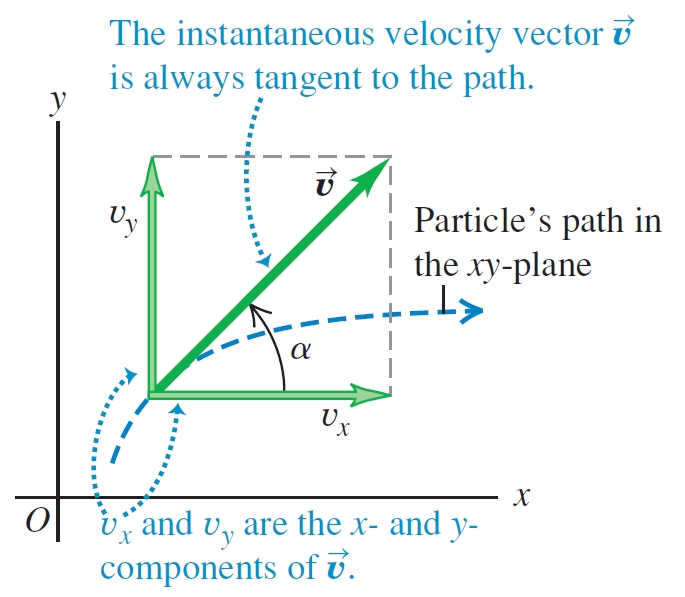
\includegraphics[width=0.8\textwidth]{images/10.jpg}
        \caption{ {\tiny Figure from Sears and Zemansky's University Physics 
        with Modern Physics, 13th Edition.} }
     \end{figure}
     
     
     
        \end{columns}



\end{frame}



%%%%%%%%%%%%%%%%%%%%%%%%%%%%%%%%%%%%%%%%%%%%%%%%%%%%%%%%%%%%%%%%%%%

\begin{frame}
EXERCISE 3.3

    \vspace{3mm}

A robotic vehicle, or rover, is exploring the surface of Mars. The
stationary Mars lander is the origin of coordinates, and the surrounding
Martian surface lies in the xy-plane. The rover, which we
represent as a point, has x- and y-coordinates that vary with time:
 

  \vspace{3mm}

         \begin{equation}
  x=(2.00-0.25t^2)~m
         \end{equation}

         \begin{equation}
  y=(t+0.025t^3)~m
         \end{equation}

 \vspace{3mm}

(a) Find the rover’s coordinates and distance from the lander at $t=2~s$.
(b) Find the rover’s displacement and average velocity
vectors for the interval $t=0~s$ to $t=2~s$.

\end{frame}

%%%%%%%%%%%%%%%%%%%%%%%%%%%%%%%%%%%%%%%%%%%%%%%%%%%%%%%%%%%%%%%%%%%

%\begin{frame}
%TEST YOUR UNDERSTANDING

%    \vspace{3mm}

%In which of these situations would the average velocity vector $\vec{v}_{av}$  over an interval be equal to the instantaneous
%velocity $\vec{v}$ at the end of the interval?


%    \vspace{3mm}

%\begin{enumerate}
%\item a body moving along a curved path
%at constant speed;
%\item a body moving along a curved path and speeding up;
%\item a body
%moving along a straight line at constant speed;
%\item a body moving along a straight line
%and speeding up.
%\end{enumerate}

%\end{frame}


%%%%%%%%%%%%%%%%%%%%%%%%%%%%%%%%%%%%%%%%%%%%%%%%%%%%%%%%%%%%%%%%%%%




\begin{frame}
The Instantaneous acceleration  is,

    \vspace{3mm}

         \begin{equation}
          \vec{a}=\frac{dv_x}{dt}\hat{\imath}+\frac{dv_y}{dt}\hat{\jmath}+\frac{dv_z}{dt}\hat{k}
         \end{equation}
   \vspace{3mm}
where,

   \begin{equation}
       a_x=\frac{dv_yx}{dt},~ a_y=\frac{dv_y}{dt}~and~a_z=\frac{dv_z}{dt}
         \end{equation}

        \vspace{3mm}
Its magnitude is,


        \vspace{3mm}



         \begin{equation}
          |\vec{a}|=\sqrt{a^2_x+a^2_y+a^2_z}
         \end{equation}




\end{frame}

%%%%%%%%%%%%%%%%%%%%%%%%%%%%%%%%%%%%%%%%%%%%%%%%%%%%%%%%%%%%%%%%%%%



\begin{frame}

    Parallel and Perpendicular Components of Acceleration
    
    \vspace{3mm}


    \begin{columns}[c]
        \column{2in}  % slides are 3in high by 5in wide
       

        A useful way to think about the acceleration
        is in terms of its component parallel to the  path and its component perpendicular 
        to the  path.



        \column{2.5in}
        
        \begin{figure}[h!]  
       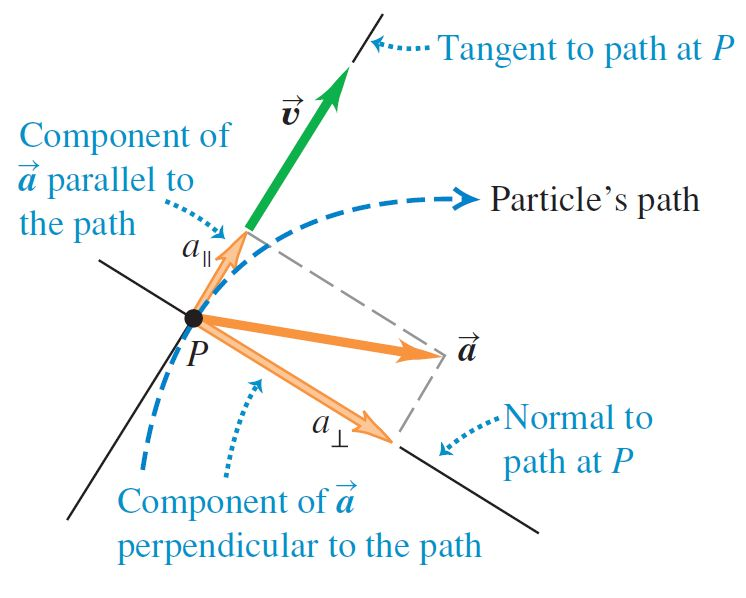
\includegraphics[width=0.9\textwidth]{images/11.jpg}
        \caption{ {\tiny Figure from Sears and Zemansky's University Physics 
        with Modern Physics, 13th Edition.} }
     \end{figure}
     
     
     
        \end{columns}



\end{frame}




%%%%%%%%%%%%%%%%%%%%%%%%%%%%%%%%%%%%%%%%%%%%%%%%%%%%%%%%%%%%%%%%%%%



\begin{frame}

  

   

 
        \begin{figure}[h!]  
            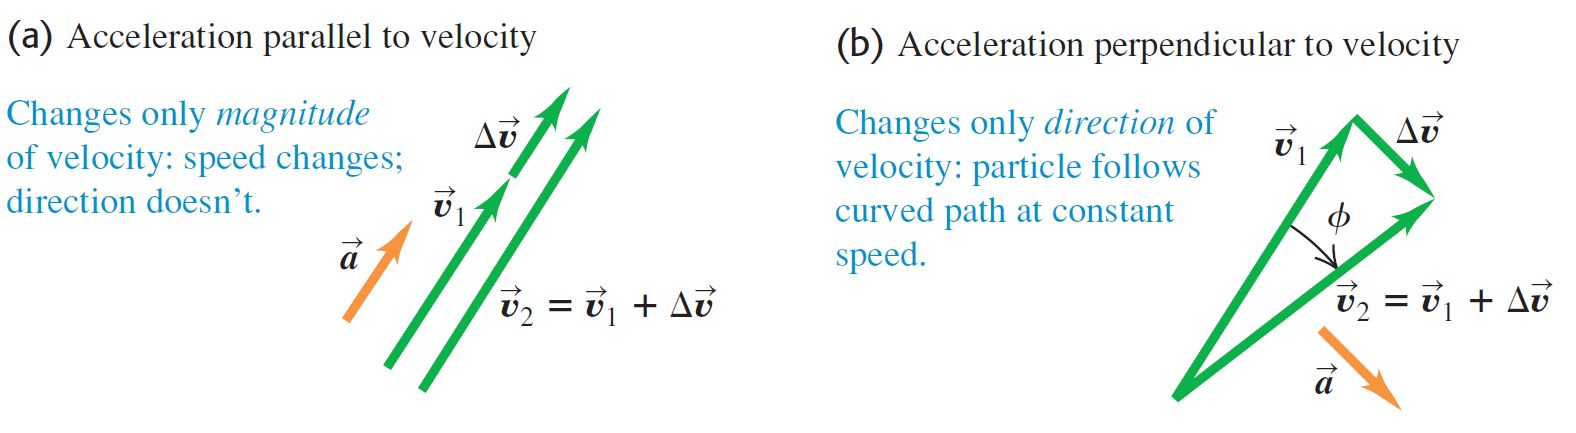
\includegraphics[width=1.\textwidth]{images/12.jpg}
             \caption{ {\tiny Figure from Sears and Zemansky's University Physics 
             with Modern Physics, 13th Edition.} }
          \end{figure}

\end{frame}



%%%%%%%%%%%%%%%%%%%%%%%%%%%%%%%%%%%%%%%%%%%%%%%%%%%%%%%%%%%%%%%%%%%



\begin{frame}

  

   

 
    \begin{figure}[h!]  
        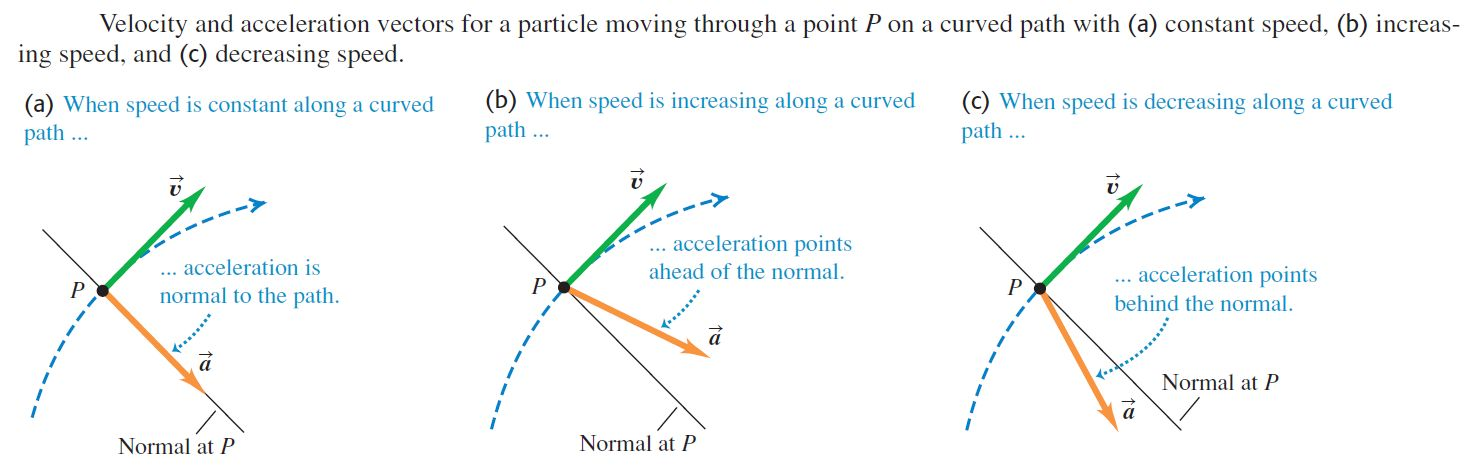
\includegraphics[width=1.2\textwidth]{images/13.jpg}
         \caption{ {\tiny Figure from Sears and Zemansky's University Physics 
         with Modern Physics, 13th Edition.} }
      \end{figure}

\end{frame}





%%%%%%%%%%%%%%%%%%%%%%%%%%%%%%%%%%%%%%%%%%%%%%%%%%%%%%%%%%%%%%%%%%%



\begin{frame}
    Conceptual Example:
    \vspace{3mm}


      \begin{columns}[c]
          \column{2in}  % slides are 3in high by 5in wide
         
  
          A skier moves along a ski-jump ramp. The ramp is
          straight from point A to point C and curved from point C onward.
          The skier speeds up as she moves downhill from point A to point E,
          where her speed is maximum. She slows down after passing point
          E. Draw the direction of the acceleration vector at each of the
          points B, D, E, and F.
      
  
  
          \column{2.5in}
          
          \begin{figure}[h!]  
         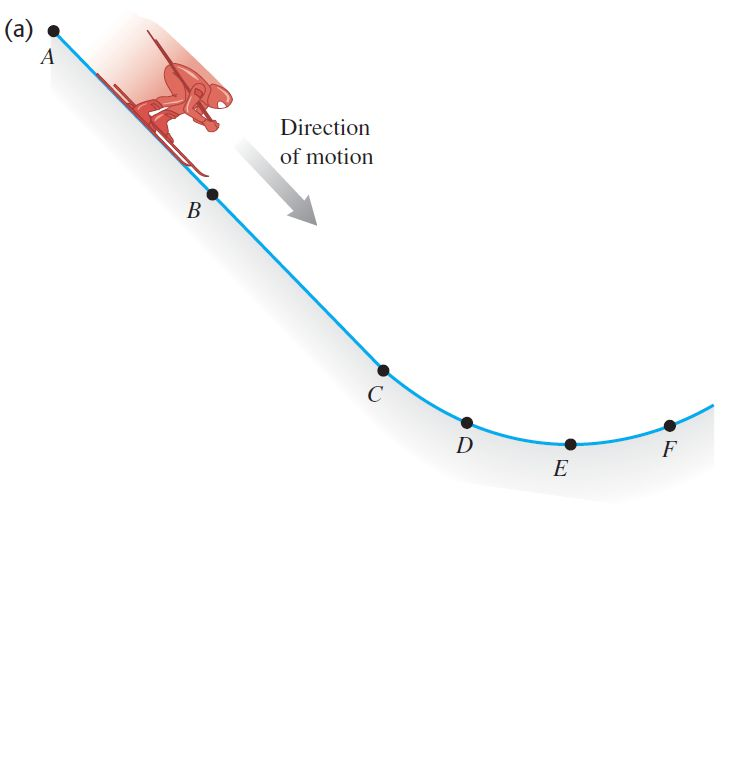
\includegraphics[width=0.9\textwidth]{images/15.jpg}
          \caption{ {\tiny Figure from Sears and Zemansky's University Physics 
          with Modern Physics, 13th Edition.} }
       \end{figure}
       
       
       
          \end{columns}

          


\end{frame}



%%%%%%%%%%%%%%%%%%%%%%%%%%%%%%%%%%%%%%%%%%%%%%%%%%%%%%%%%%%%%%%%%%%



\begin{frame}
    Conceptual Example:
    \vspace{3mm}


      \begin{columns}[c]
          \column{2in}  % slides are 3in high by 5in wide
         
  
          A skier moves along a ski-jump ramp. The ramp is
          straight from point A to point C and curved from point C onward.
          The skier speeds up as she moves downhill from point A to point E,
          where her speed is maximum. She slows down after passing point
          E. Draw the direction of the acceleration vector at each of the
          points B, D, E, and F.
      
  
  
          \column{2.5in}
          
          \begin{figure}[h!]  
         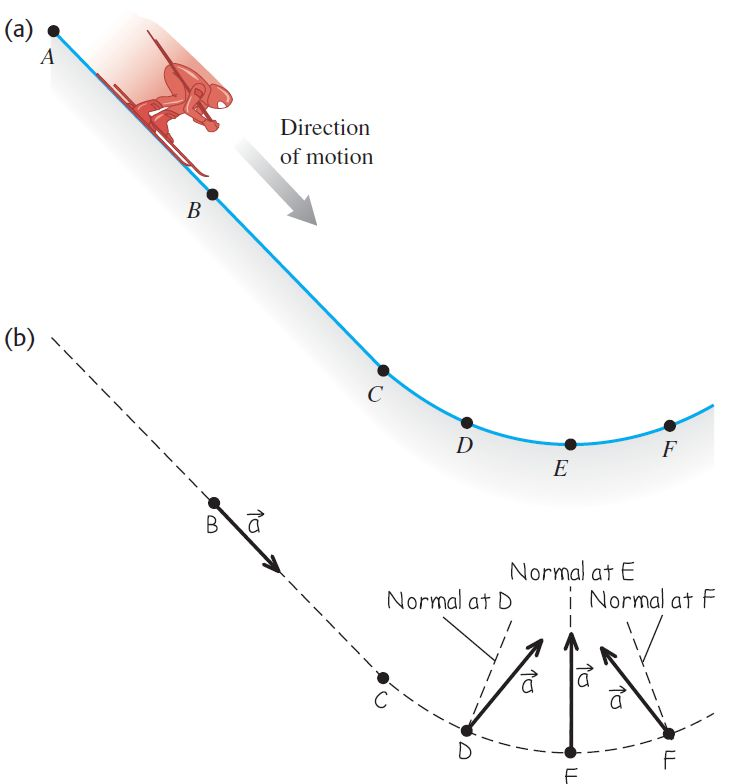
\includegraphics[width=0.9\textwidth]{images/14.jpg}
          \caption{ {\tiny Figure from Sears and Zemansky's University Physics 
          with Modern Physics, 13th Edition.} }
       \end{figure}
       
       
       
          \end{columns}

          


\end{frame}


%%%%%%%%%%%%%%%%%%%%%%%%%%%%%%%%%%%%%%%%%%%%%%%%%%%%%%%%%%%%%%%%%%%



\begin{frame}
    Test Your Undertanding
    \vspace{3mm}


      \begin{columns}[c]
          \column{2in}  % slides are 3in high by 5in wide
         
          A sled travels over
          the crest of a snow-covered hill. The
          sled slows down as it climbs up one
          side of the hill and gains speed as it
          descends on the other side. Which of
          the vectors (1 through 9) in the figure
          correctly shows the direction of the
          sled’s acceleration at the crest? (Choice 9 is that the acceleration is zero.)
      
  
  
          \column{2.5in}
          
          \begin{figure}[h!]  
         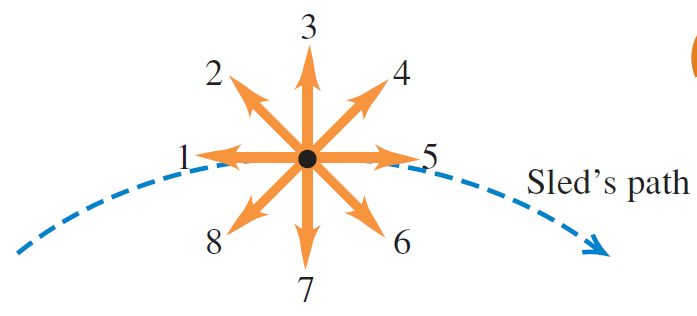
\includegraphics[width=0.9\textwidth]{images/17.jpg}
          \caption{ {\tiny Figure from Sears and Zemansky's University Physics 
          with Modern Physics, 13th Edition.} }
       \end{figure}
       
       
       
          \end{columns}

          


\end{frame}



%%%%%%%%%%%%%%%%%%%%%%%%%%%%%%%%%%%%%%%%%%%%%%%%%%%%%%%%%%%%%%%%%%%
\subsection{Projectile Motion}


\begin{frame}
    Projectile Motion  
    \vspace{3mm}

    A projectile is any body that is given an initial velocity and then follows a path
    determined entirely by the effects of gravitational acceleration and air resistance.
    \vspace{3mm}

     The path followed by a projectile is
    called its trajectory.

    

          


\end{frame}


%%%%%%%%%%%%%%%%%%%%%%%%%%%%%%%%%%%%%%%%%%%%%%%%%%%%%%%%%%%%%%%%%%%


\begin{frame}
Projectile Motion  
  \vspace{3mm}

    
      \begin{columns}[c]
          \column{2.3in}  % slides are 3in high by 5in wide
         
    \begin{itemize}
        \item we can treat the x- and
        y-coordinates separately.
        \item The x-component of acceleration is zero, and the
        y-component is constant and equal to $-g$
        \item So,  projectile
        motion is a combination of horizontal motion with constant velocity and
        vertical motion with constant acceleration.
    \end{itemize}

  
  
          \column{2.5in}
          
          \begin{figure}[h!]  
         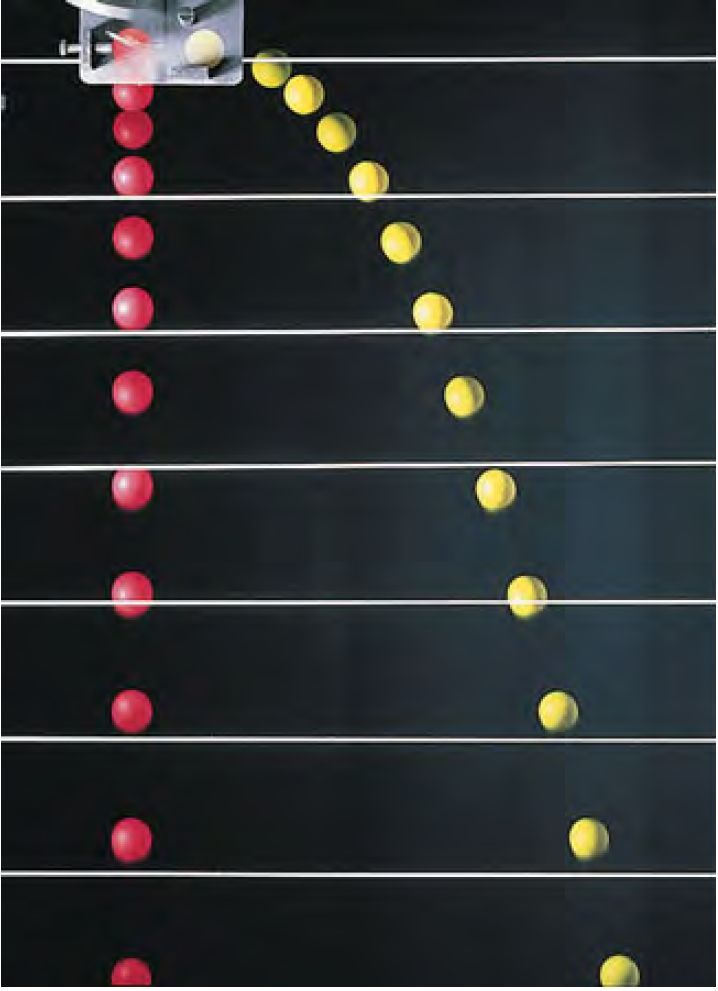
\includegraphics[width=0.7\textwidth]{images/18.jpg}
          \caption{ {\tiny Figure from Sears and Zemansky's University Physics 
          with Modern Physics, 13th Edition.} }
       \end{figure}
       
       
       
          \end{columns}

          


\end{frame}



%%%%%%%%%%%%%%%%%%%%%%%%%%%%%%%%%%%%%%%%%%%%%%%%%%%%%%%%%%%%%%%%%%%


\begin{frame}
   
  

  \begin{equation}
    x-motion:\ \ \  x=v_{x0}t+x_0
  \end{equation}
  

  \begin{equation}
    y-motion: \ \ \ y=-\frac{1}{2}gt^ 2+v_{y0}t+y_0
  \end{equation}

  \begin{figure}[h!]  
    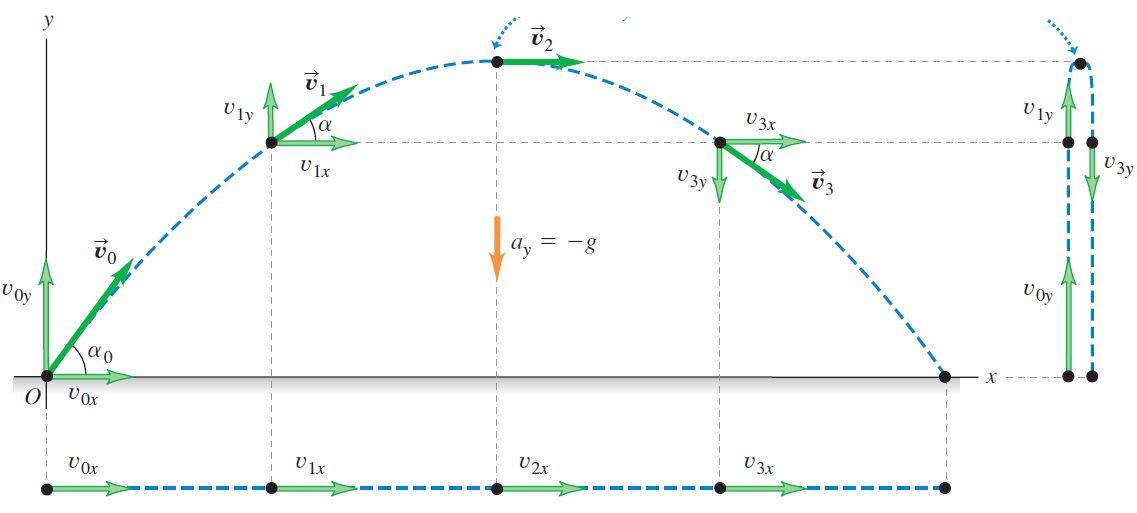
\includegraphics[width=0.9\textwidth]{images/19.jpg}
     \caption{ {\tiny Figure from Sears and Zemansky's University Physics 
     with Modern Physics, 13th Edition.} }
  \end{figure}
   


\end{frame}


%%%%%%%%%%%%%%%%%%%%%%%%%%%%%%%%%%%%%%%%%%%%%%%%%%%%%%%%%%%%%%%%%%%


\begin{frame}
   
  



    \begin{columns}[c]
        \column{2.3in}  % slides are 3in high by 5in wide
       
        \begin{equation*}
            v_{x0}=? \ \ \  v_{y0}=?
          \end{equation*}
          
        
      
      

        \column{2.5in}
        
  
        \begin{figure}[h!]  
            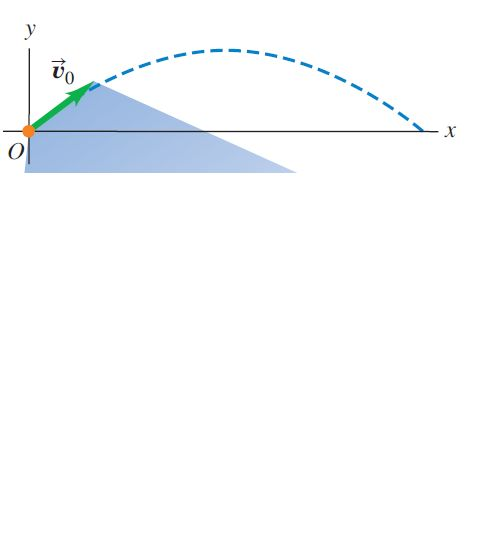
\includegraphics[width=0.7\textwidth]{images/20_0.jpg}
         
          \end{figure}
           
     
        \end{columns}



  
  \end{frame}
  
%%%%%%%%%%%%%%%%%%%%%%%%%%%%%%%%%%%%%%%%%%%%%%%%%%%%%%%%%%%%%%%%%%%


\begin{frame}
   
  


  


    \begin{columns}[c]
        \column{2.3in}  % slides are 3in high by 5in wide
       

        \begin{equation*}
            v_{x0}=v_0cos\alpha_0, \ \ \  v_{y0}=v_0sin\alpha_0
          \end{equation*}
          
        
          \begin{equation*}
        tan \alpha_0=\frac{v_{x0}}{v_{y0}}
          \end{equation*}
        
      

        \column{2.5in}
        
  
        \begin{figure}[h!]  
            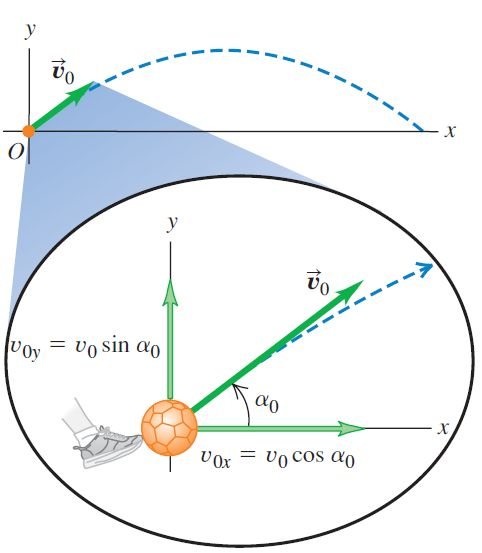
\includegraphics[width=0.7\textwidth]{images/20.jpg}
             \caption{ {\tiny Figure from Sears and Zemansky's University Physics 
             with Modern Physics, 13th Edition.} }
          \end{figure}
           
     
        \end{columns}

     
    
            
  
  \end{frame}
  





%%%%%%%%%%%%%%%%%%%%%%%%%%%%%%%%%%%%%%%%%%%%%%%%%%%%%%%%%%%%%%%%%%%


\begin{frame}
   
  
    \begin{figure}[h!]  
        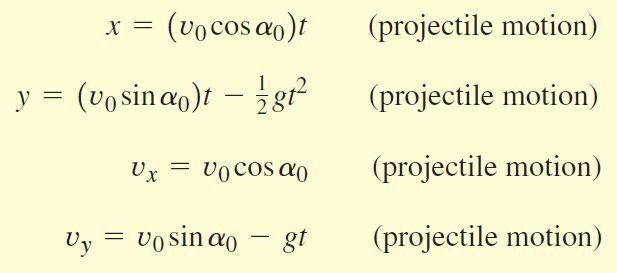
\includegraphics[width=0.7\textwidth]{images/21.jpg}
         \caption{ {\tiny Table from Sears and Zemansky's University Physics 
         with Modern Physics, 13th Edition.} }
      \end{figure}
       

    
  
  \end{frame}




%%%%%%%%%%%%%%%%%%%%%%%%%%%%%%%%%%%%%%%%%%%%%%%%%%%%%%%%%%%%%%%%%%%


\begin{frame}
   
    Motion Path?
   \pause

       \begin{equation*}
           y(x)=(tan \alpha_0)x-\frac{g}{2v^2_0cos^2\alpha_0}x^2
           \end{equation*}
   
    \pause     

  PARABOLA

    \pause     


 \begin{equation*}
     \rightarrow      y(x)=bx-cx^2 \ \ \ parabola
\end{equation*}
     
     \end{frame}


%%%%%%%%%%%%%%%%%%%%%%%%%%%%%%%%%%%%%%%%%%%%%%%%%%%%%%%%%%%%%%%%%%%


\begin{frame}
   
  What if we include air resistance?
   \pause


           \begin{figure}[h!]  
            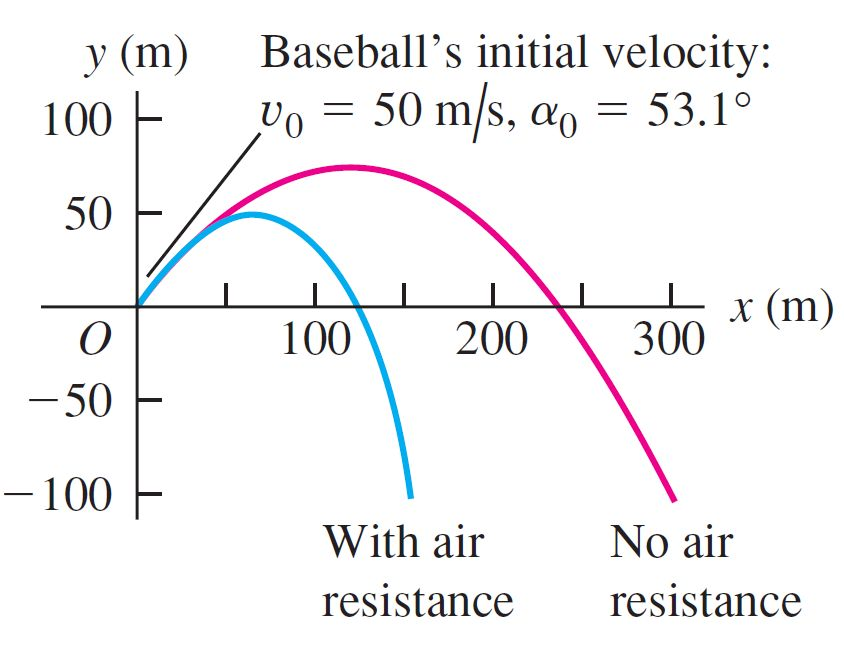
\includegraphics[width=0.7\textwidth]{images/22.jpg}
             \caption{ {\tiny Table from Sears and Zemansky's University Physics 
             with Modern Physics, 13th Edition.} }
          \end{figure}
            

     
     \end{frame}




%%%%%%%%%%%%%%%%%%%%%%%%%%%%%%%%%%%%%%%%%%%%%%%%%%%%%%%%%%%%%%%%%%%


\begin{frame}
    HEIGHT AND RANGE OF A PROJECTILE

    \vspace{3mm}

  \pause


  A batter hits a baseball so that it leaves the bat at speed $v_0=37~m/s$
at an angle $\alpha_0=53.1^{\circ}$. Find: 
\vspace{3mm}

\begin{enumerate}
    \item the time for  the highest point, and its
    height $h$ at this times
    \item   the horizontal range $R$  
\end{enumerate}
    

    
\vspace{3mm}

\begin{figure}[h!]  
    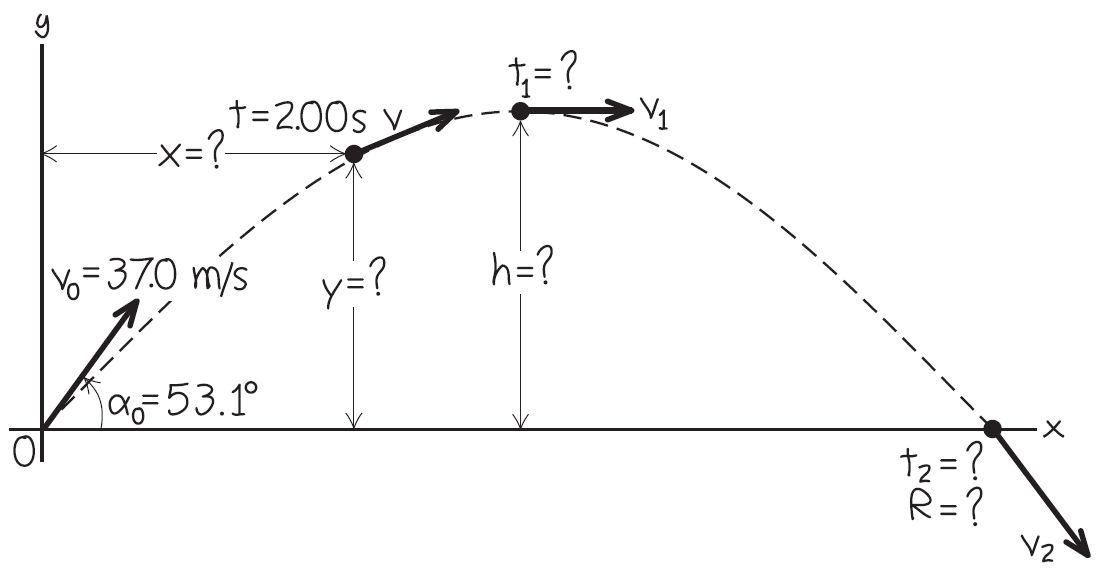
\includegraphics[width=0.7\textwidth]{images/23.jpg}
     \caption{ {\tiny Table from Sears and Zemansky's University Physics 
     with Modern Physics, 13th Edition.} }
  \end{figure}
    

       
       \end{frame}





%%%%%%%%%%%%%%%%%%%%%%%%%%%%%%%%%%%%%%%%%%%%%%%%%%%%%%%%%%%%%%%%%%%


\begin{frame}

  HEIGHT
    \vspace{3mm}

\begin{equation*}
v_y=v_{0y}-gt=0\rightarrow t=\frac{v_{0}sin\ \alpha_0}{g}
\end{equation*} 

\vspace{3mm}

\pause

\begin{equation*}
    h=v_{0y}t-\frac{1}{2}gt^2
\end{equation*} 


\pause



\vspace{3mm}

\pause

\begin{equation*}
\rightarrow  h=\frac{v_{0}^2sin \ \alpha^2_0}{2g}
\end{equation*} 

\vspace{3mm}

\pause

EXTRA-CREDIT: PROOF IT
       
\end{frame}




%%%%%%%%%%%%%%%%%%%%%%%%%%%%%%%%%%%%%%%%%%%%%%%%%%%%%%%%%%%%%%%%%%%


\begin{frame}

    RANGE
      \vspace{3mm}
  
  \begin{equation*}
t_{l}=2\frac{v_{0}sin{\ \alpha_0}}{g}
  \end{equation*} 

  \begin{equation*}
R=v_{0x}t=2v_{0x}\frac{v_{0}sin{\ \alpha_0}}{g}=2v_{0}cos\ \alpha\frac{v_{0}sin{\ \alpha_0}}{g}
      \end{equation*} 

\begin{equation*}
 \rightarrow   R=\frac{v^2_{0}sin{\ 2\alpha_0}}{g}
\end{equation*}      

  \end{frame}
  

%%%%%%%%%%%%%%%%%%%%%%%%%%%%%%%%%%%%%%%%%%%%%%%%%%%%%%%%%%%%%%%%%%%


\begin{frame}

VARIATION OF RANGE WITH INITIAL INCLINATION
\vspace{3mm}

\begin{figure}[h!]  
    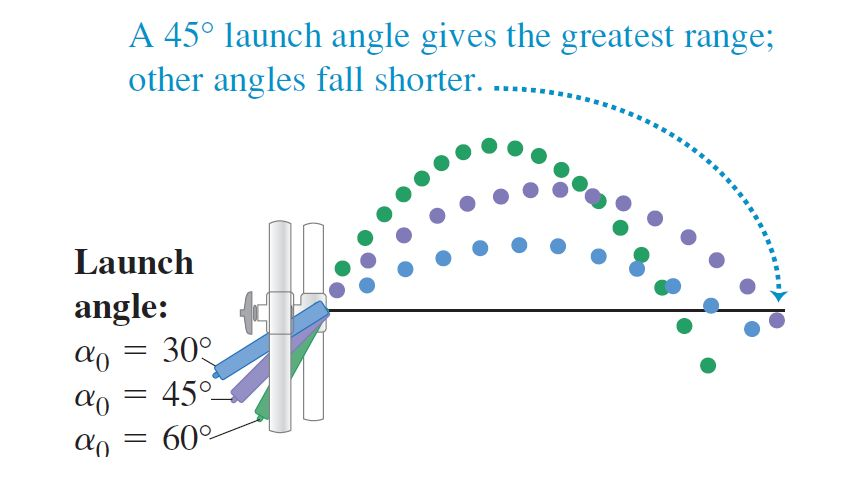
\includegraphics[width=0.7\textwidth]{images/24.jpg}
     \caption{ {\tiny Figure from Sears and Zemansky's University Physics 
     with Modern Physics, 13th Edition.} }
  \end{figure}

  \end{frame}
  




%%%%%%%%%%%%%%%%%%%%%%%%%%%%%%%%%%%%%%%%%%%%%%%%%%%%%%%%%%%%%%%%%%%


\begin{frame}

    A classic Physics problem: "The zookeeper and the monkey"
    
    \vspace{3mm}
    
    \begin{figure}[h!]  
        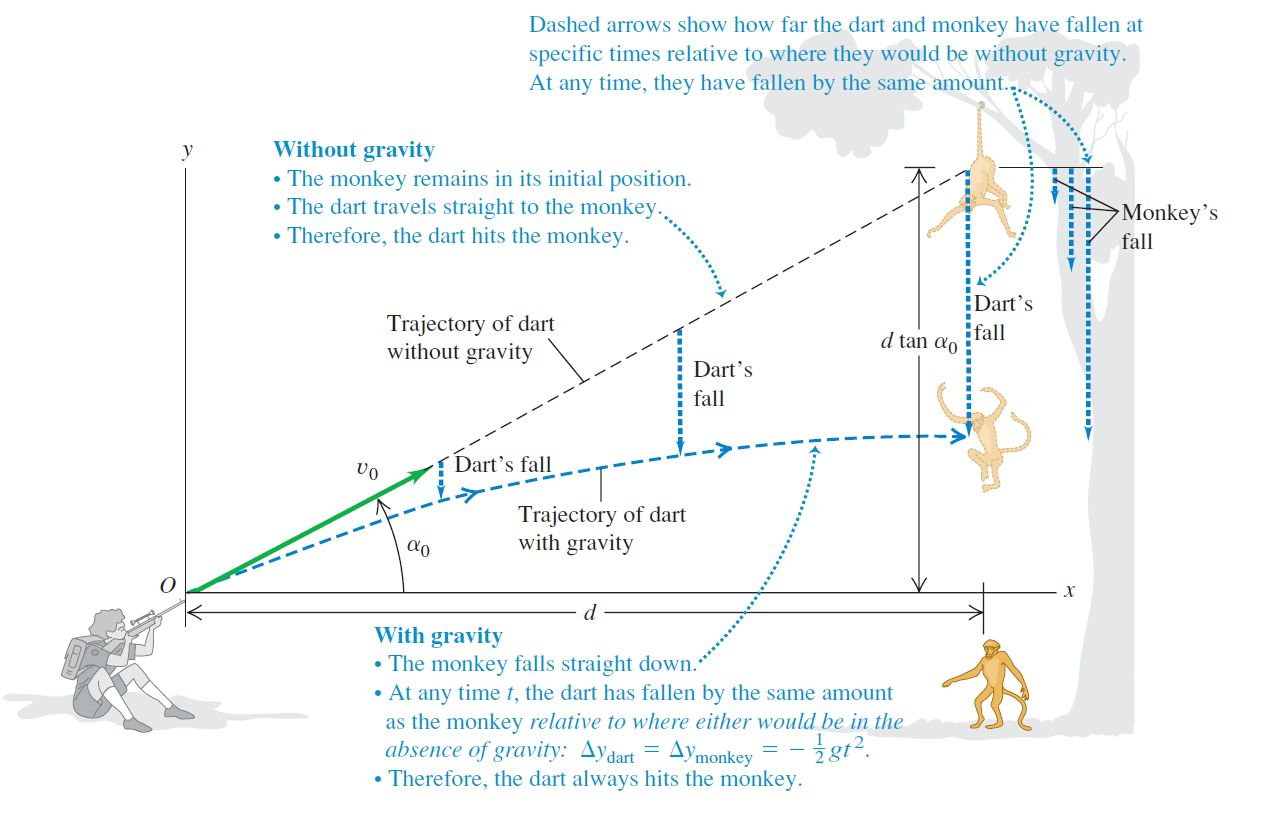
\includegraphics[width=0.9\textwidth]{images/25.jpg}
         \caption{ {\tiny Figure from Sears and Zemansky's University Physics 
         with Modern Physics, 13th Edition.} }
      \end{figure}
    
      \end{frame}


%%%%%%%%%%%%%%%%%%%%%%%%%%%%%%%%%%%%%%%%%%%%%%%%%%%%%%%%%%%%%%%%%%%


\begin{frame}

  
DART:
    \begin{equation*}
       x_d=v_{0x}t
       \end{equation*}     
       \begin{equation*}
        y_d=v_{0y}t-(\frac{1}{2})gt^2
        \end{equation*}    

        \vspace{5mm}
        MONKEY:   
    \begin{equation*}
        x_m=D
        \end{equation*}  

        \begin{equation*}
         y_m=-(\frac{1}{2})gt^2+H
         \end{equation*}    

      \end{frame}
      
%%%%%%%%%%%%%%%%%%%%%%%%%%%%%%%%%%%%%%%%%%%%%%%%%%%%%%%%%%%%%%%%%%%


\begin{frame}

  
        \begin{equation*}
         \rightarrow tan\  \alpha=\frac{H}{D}
        \end{equation*}     
    
        
          \pause

          \vspace{5mm}

The dart is going to hit the monkey as long the  zookeeper points right to the monkey at the begining.

\pause
\vspace{5mm}

EXTRA-CREDIT: PROOF IT


\end{frame}
%%%%%%%%%%%%%%%%%%%%%%%%%%%%%%%%%%%%%%%%%%%%%%%%%%%%%%%%%%%%%%%%%%%


\begin{frame}

    Suppose the tranquilizer dart
    has a relatively low muzzle velocity so that
    the dart reaches a maximum height at a
    point P before striking the monkey,
    as shown in the figure. When the
    dart is at point P, will the monkey
    be (i) at point A (higher than P),
    (ii) at point B (at the same height
    as P), or (iii) at point C (lower
    than P)? Ignore air resistance.

    \vspace{3mm}
    
    \begin{figure}[h!]  
        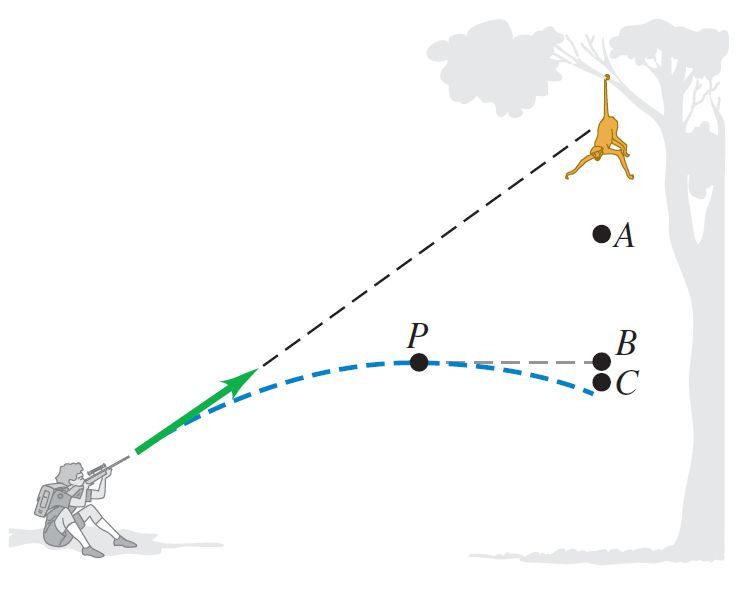
\includegraphics[width=0.5\textwidth]{images/26.jpg}
         \caption{ {\tiny Figure from Sears and Zemansky's University Physics 
         with Modern Physics, 13th Edition.} }
      \end{figure}


    
      \end{frame}
      




%%%%%%%%%%%%%%%%%%%%%%%%%%%%%%%%%%%%%%%%%%%%%%%%%%%%%%%%%%%%%%%%%%%
\subsection{ Circular Motion}
%%%%%%%%%%%%%%%%%%%%%%%%%%%%%%%%%%%%%%%%%%%%%%%%%%%%%%%%%%%%%%%%%%%

\begin{frame}

   Uniform Circular Motion
   \vspace{3mm}
   
   \begin{itemize}
   \item Motion in a circle with constant speed.
    \item There is no component of acceleration parallel (tangent) to the path.
\item The acceleration vector is perpendicular to the path and hence directed inward.
\item This causes the direction of the velocity to change without changing the speed
   \end{itemize}

    
      \end{frame}
      
%%%%%%%%%%%%%%%%%%%%%%%%%%%%%%%%%%%%%%%%%%%%%%%%%%%%%%%%%%%%%%%%%%%




\begin{frame}

    \begin{figure}[h!]  
        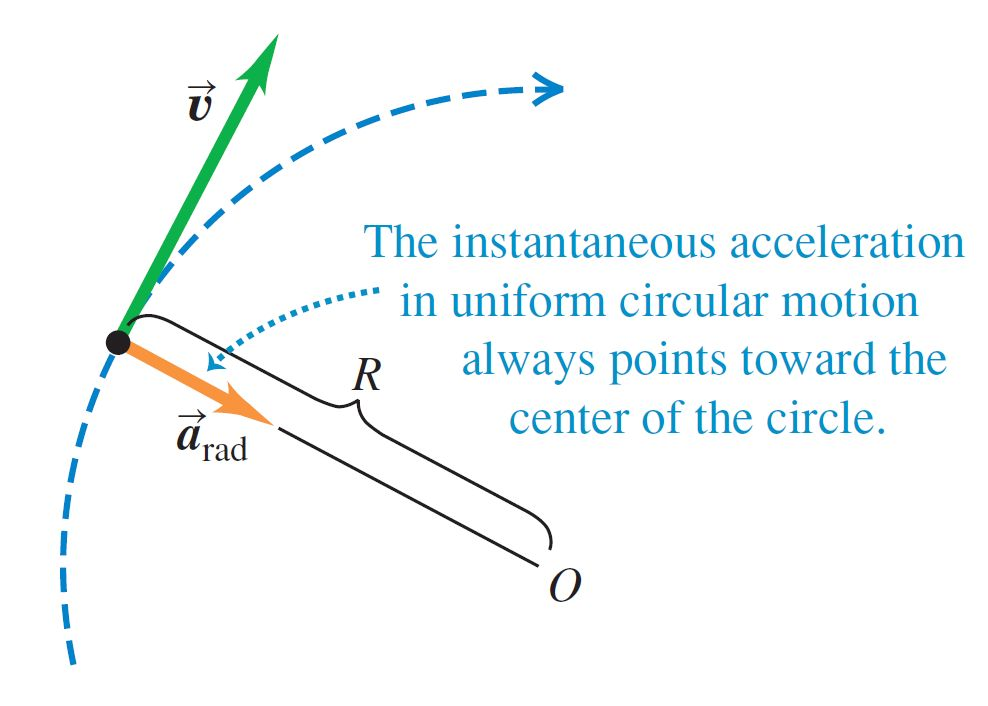
\includegraphics[width=0.8\textwidth]{images/28.jpg}
        \caption{ {\tiny Figure from Sears and Zemansky's University Physics 
        with Modern Physics, 13th Edition.} }
      \end{figure}
      
      
      
     
       \end{frame}
       

%%%%%%%%%%%%%%%%%%%%%%%%%%%%%%%%%%%%%%%%%%%%%%%%%%%%%%%%%%%%%%%%%%%




\begin{frame}
    Magnitude of $\vec{a}$?
 
   
   \begin{columns}[c]
        \column{2.3in}  % slides are 3in high by 5in wide
       
     

        \begin{equation*}
           \Delta \Phi R =\Delta s 
          \end{equation*}
          
        


        \column{2.5in}
        
  
        \begin{figure}[h!]  
            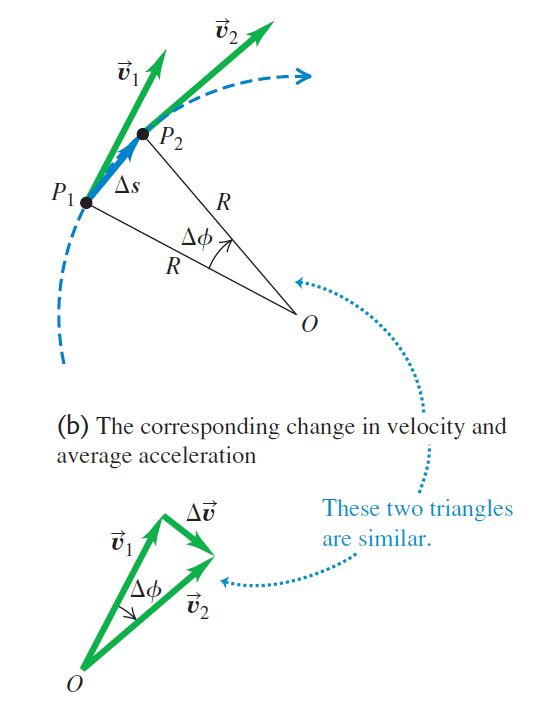
\includegraphics[width=0.8\textwidth]{images/27.jpg}
            \caption{ {\tiny Figure from Sears and Zemansky's University Physics 
            with Modern Physics, 13th Edition.} }
          \end{figure}
		  
		  
		  
           
     
        \end{columns}

    
      \end{frame}
      






%%%%%%%%%%%%%%%%%%%%%%%%%%%%%%%%%%%%%%%%%%%%%%%%%%%%%%%%%%%%%%%%%%%




\begin{frame}

    Magnitude of $\vec{a}$?
   
    \begin{columns}[c]
         \column{2.3in}  % slides are 3in high by 5in wide
        
        


         \begin{equation*}
            \Delta \Phi R =\Delta s 
           \end{equation*}
           
         
            \begin{equation*}
            \Delta \Phi v_1 =\vert \Delta  \vec{v} \vert \rightarrow \frac{\vert\Delta \vec{v}\vert}{v_1} =\frac{\Delta s}{R}
           \end{equation*}
  

 
         \column{2.5in}
         
   
         \begin{figure}[h!]  
             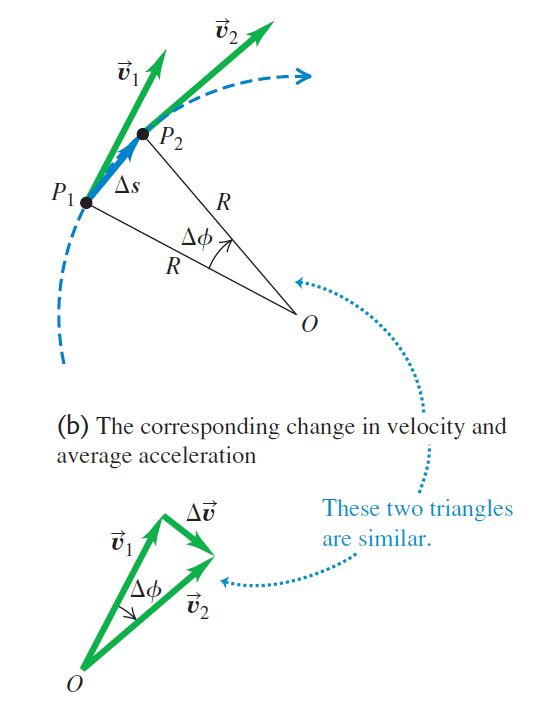
\includegraphics[width=0.8\textwidth]{images/27.jpg}
             \caption{ {\tiny Figure from Sears and Zemansky's University Physics 
             with Modern Physics, 13th Edition.} }
           \end{figure}
           
           
           
            
      
         \end{columns}
 
     
       \end{frame}





%%%%%%%%%%%%%%%%%%%%%%%%%%%%%%%%%%%%%%%%%%%%%%%%%%%%%%%%%%%%%%%%%%%




\begin{frame}

    Magnitude of $\vec{a}$?
   
    \begin{columns}[c]
         \column{2.3in}  % slides are 3in high by 5in wide
      
         
        

         \begin{equation*}
            \Delta \Phi R =\Delta s 
           \end{equation*}
           
         
            \begin{equation*}
            \Delta \Phi v_1 =\vert \Delta  \vec{v} \vert \rightarrow \frac{\vert\Delta \vec{v}\vert}{v_1} =\frac{\Delta s}{R}
           \end{equation*}
  
         \begin{equation*}
          \vert\Delta \vec{v}\vert =v_1\frac{\Delta s}{R}\rightarrow a_{av}=\frac{v_1}{R}\frac{\Delta s}{\Delta t}
           \end{equation*}
           
     
           
 
         \column{2.5in}
         
   
         \begin{figure}[h!]  
             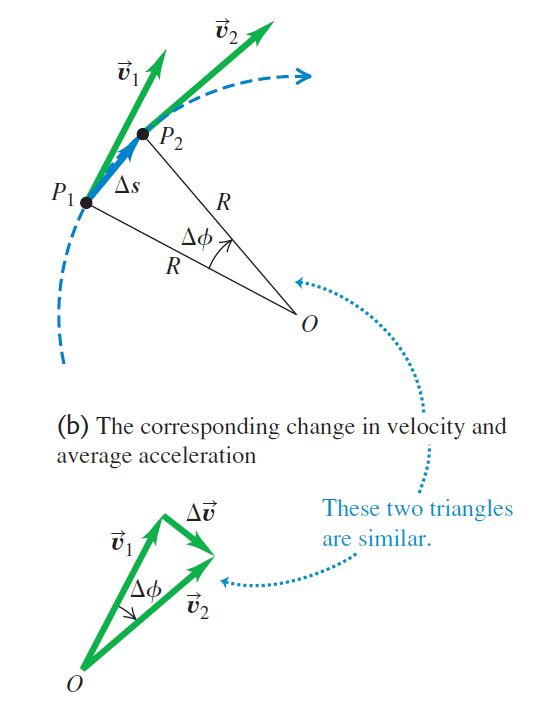
\includegraphics[width=0.8\textwidth]{images/27.jpg}
             \caption{ {\tiny Figure from Sears and Zemansky's University Physics 
             with Modern Physics, 13th Edition.} }
           \end{figure}
           
           
           
            
      
         \end{columns}
 
     
       \end{frame}





%%%%%%%%%%%%%%%%%%%%%%%%%%%%%%%%%%%%%%%%%%%%%%%%%%%%%%%%%%%%%%%%%%%




\begin{frame}

    Magnitude of $\vec{a}$?
   
    \begin{columns}[c]
         \column{2.3in}  % slides are 3in high by 5in wide
   
        


         \begin{equation*}
            \Delta \Phi R =\Delta s 
           \end{equation*}
           
         
            \begin{equation*}
            \Delta \Phi v_1 =\vert \Delta  \vec{v} \vert \rightarrow \frac{\vert\Delta \vec{v}\vert}{v_1} =\frac{\Delta s}{R}
           \end{equation*}
  
         \begin{equation*}
          \vert\Delta \vec{v}\vert =v_1\frac{\Delta s}{R}\rightarrow a_{av}=\frac{v_1}{R}\frac{\Delta s}{\Delta t}
           \end{equation*}
           
           Taking the limit for ${\Delta t\to 0}$
            \begin{equation*}
          \boxed{a=\frac{v^2}{R}}
           \end{equation*} 
           
 
         \column{2.5in}
         
   
         \begin{figure}[h!]  
             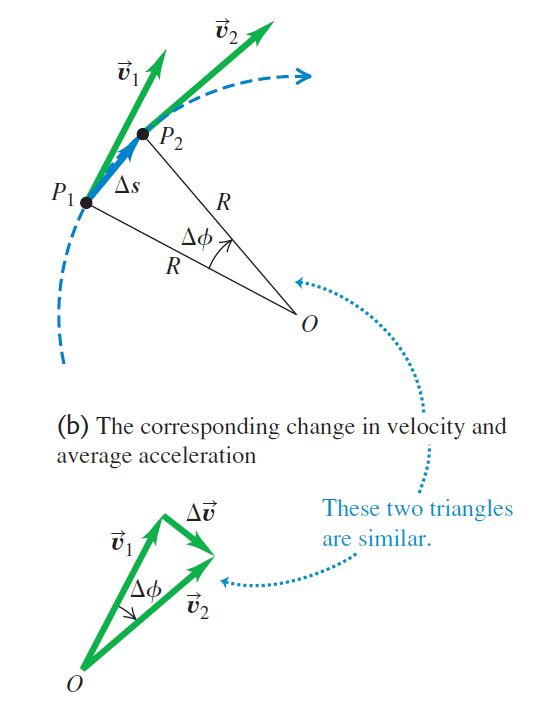
\includegraphics[width=0.8\textwidth]{images/27.jpg}
             \caption{ {\tiny Figure from Sears and Zemansky's University Physics 
             with Modern Physics, 13th Edition.} }
           \end{figure}
           
           
           
            
      
         \end{columns}
 
     
       \end{frame}

%%%%%%%%%%%%%%%%%%%%%%%%%%%%%%%%%%%%%%%%%%%%%%%%%%%%%%%%%%%%%%%%%%%




\begin{frame}

    Uniform Motion vs. Projectile Motion

            
   

         \begin{enumerate}
            \item In projectile motion, the acceleration is the same at all times.
            \item In uniform circular motion the direction of a  always points
            toward the center of the circle.
        \end{enumerate}
          

     
       \end{frame}


%%%%%%%%%%%%%%%%%%%%%%%%%%%%%%%%%%%%%%%%%%%%%%%%%%%%%%%%%%%%%%%%%%%

%%%%%%%%%%%%%%%%%%%%%%%%%%%%%%%%%%%%%%%%%%%%%%%%%%%%%%%%%%%%%%%%%%%




\begin{frame}

    Uniform Motion vs. Projectile Motion

            
   
          
         \begin{figure}[h!]  
            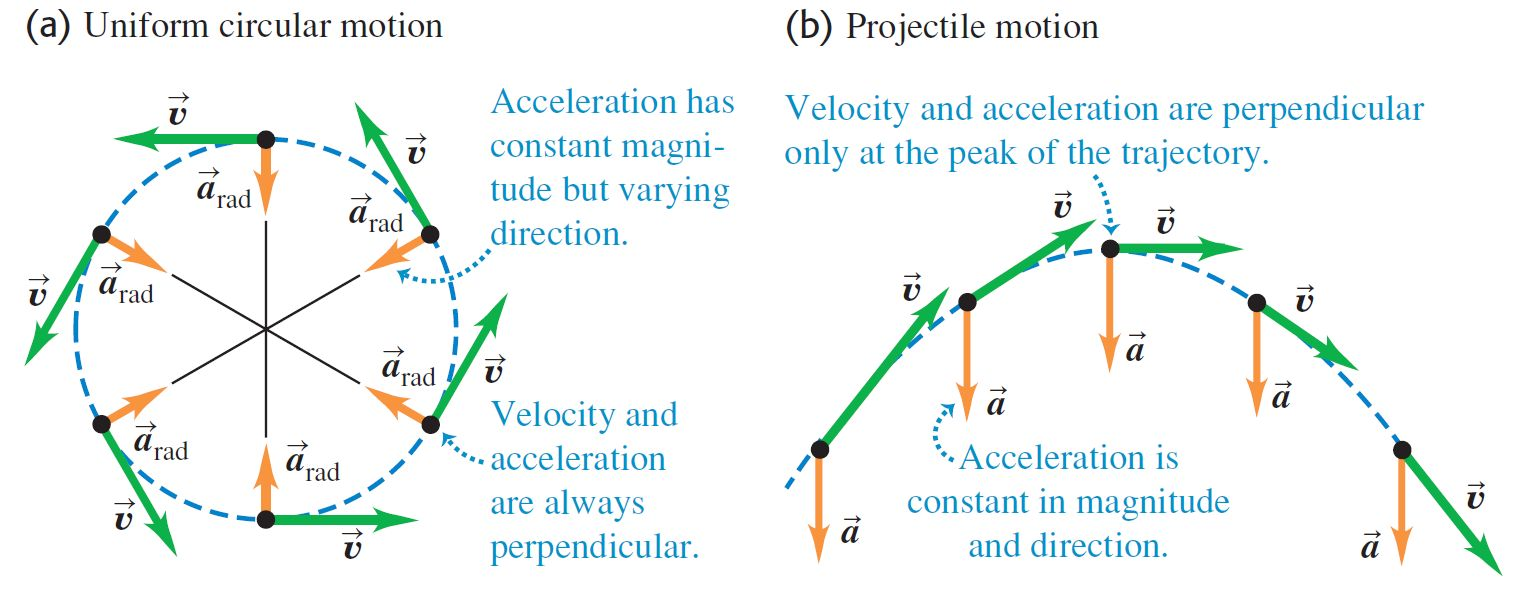
\includegraphics[width=0.9\textwidth]{images/29.jpg}
            \caption{ {\tiny Figure from Sears and Zemansky's University Physics 
            with Modern Physics, 13th Edition.} }
          \end{figure}
          
     
       \end{frame}


%%%%%%%%%%%%%%%%%%%%%%%%%%%%%%%%%%%%%%%%%%%%%%%%%%%%%%%%%%%%%%%%%%%



\begin{frame}

   Coordinates in circular motion?
   

       
  

          \begin{columns}[c]
            \column{2.3in}  % slides are 3in high by 5in wide
 
          

            \column{2.5in}
            
      
            \begin{figure}[h!]  
                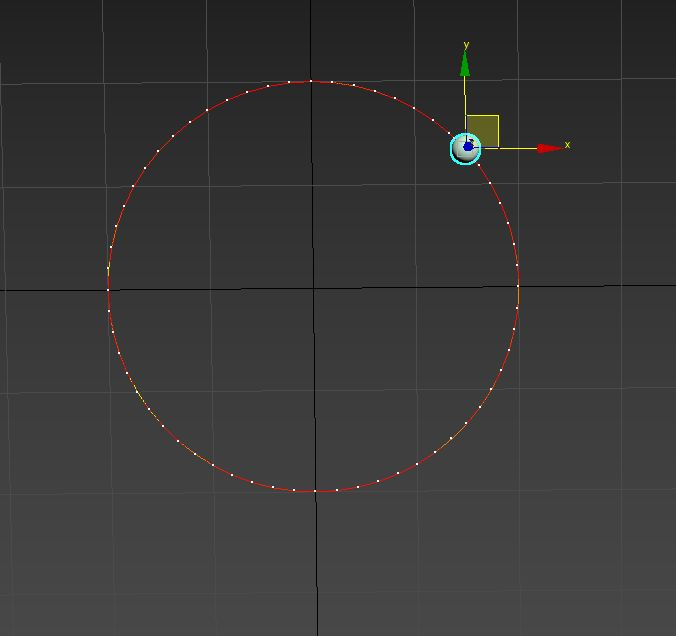
\includegraphics[width=0.8\textwidth]{images/30.jpg}
            
              \end{figure}
              
              
              
               
         
            \end{columns}



     
       \end{frame}
%%%%%%%%%%%%%%%%%%%%%%%%%%%%%%%%%%%%%%%%%%%%%%%%%%%%%%%%%%%%%%%%%%%

\begin{frame}

    Coordinates in circular motion?
    
 
        
   
 
           \begin{columns}[c]
             \column{2.3in}  % slides are 3in high by 5in wide
  
           
 
             \column{2.5in}
             
       
             \begin{figure}[h!]  
                 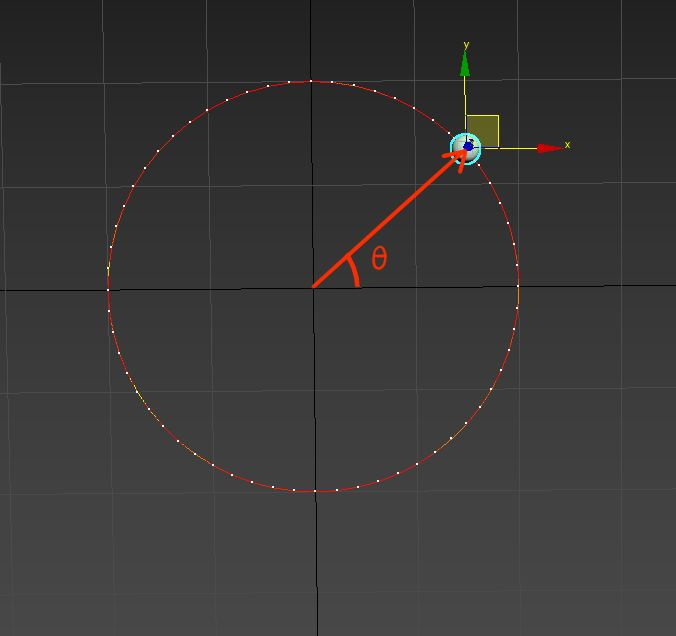
\includegraphics[width=0.8\textwidth]{images/31.jpg}
             
               \end{figure}
               
               
               
                
          
             \end{columns}
 
 
 
      
        \end{frame}
 %%%%%%%%%%%%%%%%%%%%%%%%%%%%%%%%%%%%%%%%%%%%%%%%%%%%%%%%%%%%%%%%%%%






 \begin{frame}

    Coordinates in circular motion?
    
 
        
   
 
           \begin{columns}[c]
             \column{2.3in}  % slides are 3in high by 5in wide
  
           
 
             \column{2.5in}
             
       
             \begin{figure}[h!]  
                 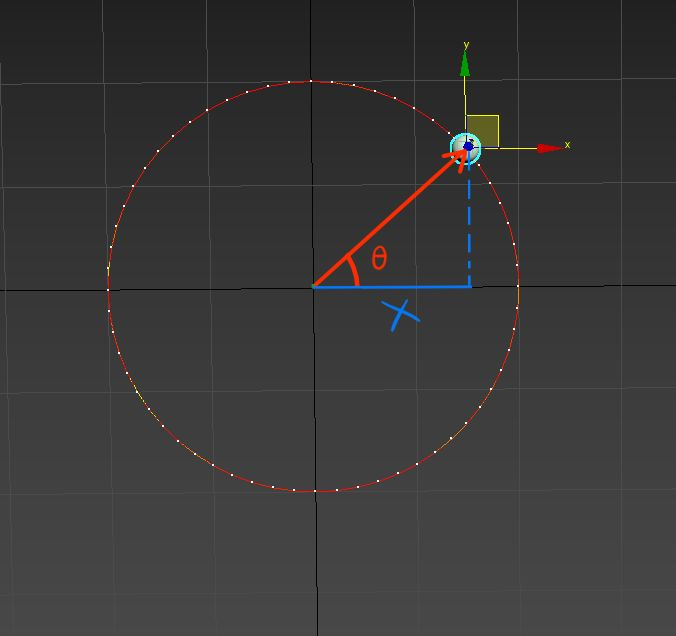
\includegraphics[width=0.8\textwidth]{images/32.jpg}
             
               \end{figure}
               
               
               
                
          
             \end{columns}
 
 
 
      
        \end{frame}
 %%%%%%%%%%%%%%%%%%%%%%%%%%%%%%%%%%%%%%%%%%%%%%%%%%%%%%%%%%%%%%%%%%%




 \begin{frame}

    Coordinates in circular motion?
    
 
        
   
 
           \begin{columns}[c]
             \column{2.3in}  % slides are 3in high by 5in wide
  
           
 
             \column{2.5in}
             
       
             \begin{figure}[h!]  
                 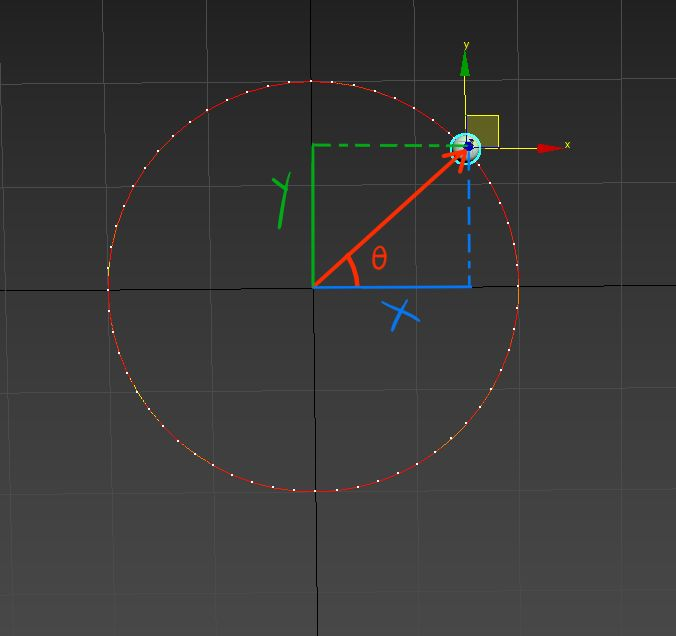
\includegraphics[width=0.8\textwidth]{images/33.jpg}
             
               \end{figure}
               
               
               
                
          
             \end{columns}
 
 
 
      
        \end{frame}
 %%%%%%%%%%%%%%%%%%%%%%%%%%%%%%%%%%%%%%%%%%%%%%%%%%%%%%%%%%%%%%%%%%%






 \begin{frame}

    Coordinates in circular motion?
    
 
        
   
 
           \begin{columns}[c]
             \column{2.3in}  % slides are 3in high by 5in wide
  
           
 
             \column{2.5in}
             
       
             \begin{figure}[h!]  
                 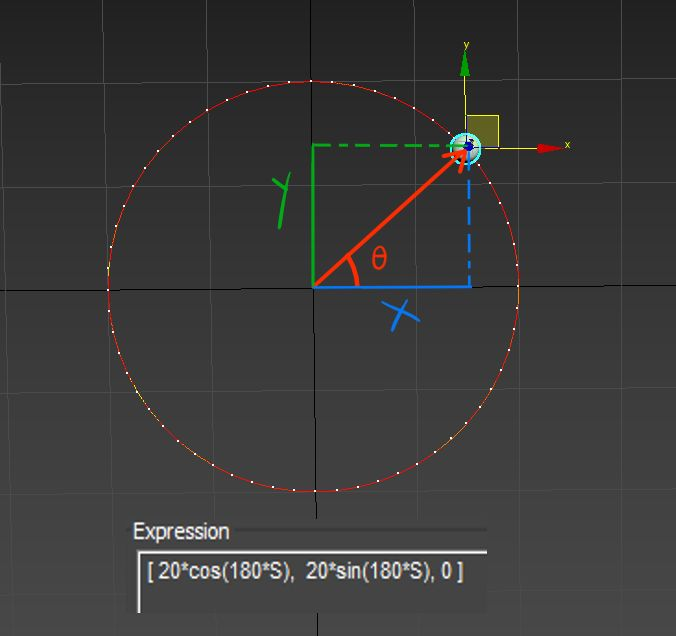
\includegraphics[width=0.8\textwidth]{images/34.jpg}
             
               \end{figure}
               
               
               
                
          
             \end{columns}
 
 
 
      
        \end{frame}
 %%%%%%%%%%%%%%%%%%%%%%%%%%%%%%%%%%%%%%%%%%%%%%%%%%%%%%%%%%%%%%%%%%%





 \begin{frame}

    Coordinates in circular motion?
    
 
        
   
 
           \begin{columns}[c]
             \column{2.3in}  % slides are 3in high by 5in wide
  
             \begin{equation*}
                x=R~cos~\theta(t)
            \end{equation*}
 
 
             \column{2.5in}
             
       
             \begin{figure}[h!]  
                 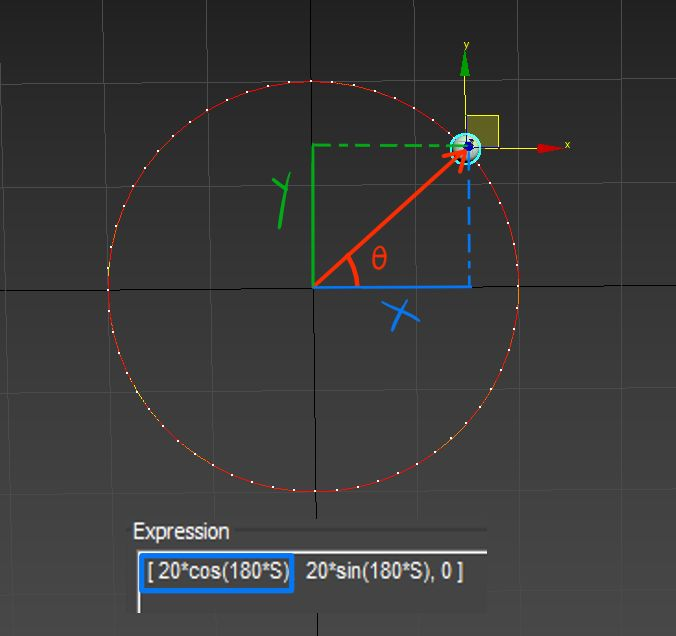
\includegraphics[width=0.8\textwidth]{images/35.jpg}
             
               \end{figure}
               
               
               
                
          
             \end{columns}
 
 
 
      
        \end{frame}
 %%%%%%%%%%%%%%%%%%%%%%%%%%%%%%%%%%%%%%%%%%%%%%%%%%%%%%%%%%%%%%%%%%%


 \begin{frame}

    Coordinates in circular motion?
    
 
        
   
 
           \begin{columns}[c]
             \column{2.3in}  % slides are 3in high by 5in wide
  
             \begin{equation*}
                x=R~cos~\theta(t)
            \end{equation*}
 

            \begin{equation*}
                y=R~sin~\theta(t)
            \end{equation*}

             \column{2.5in}
             
       
             \begin{figure}[h!]  
                 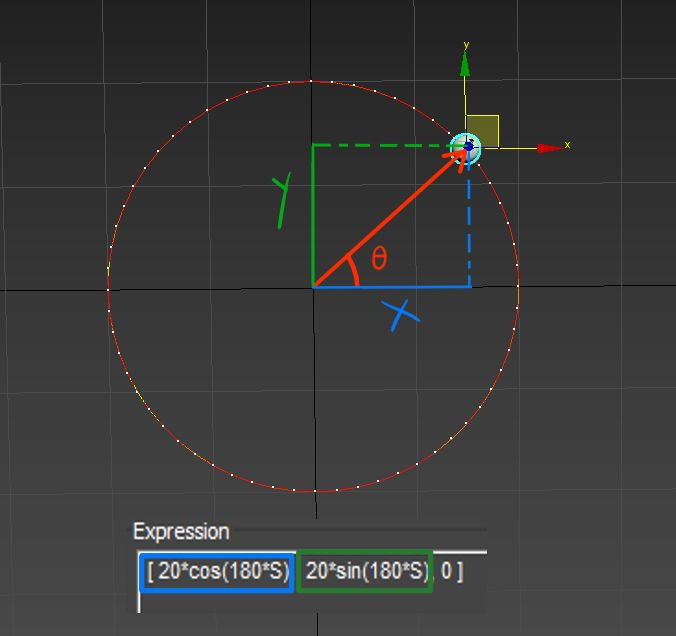
\includegraphics[width=0.8\textwidth]{images/36.jpg}
             
               \end{figure}
               
               
               
                
          
             \end{columns}
 
 
 
      
        \end{frame}
 %%%%%%%%%%%%%%%%%%%%%%%%%%%%%%%%%%%%%%%%%%%%%%%%%%%%%%%%%%%%%%%%%%%



 \begin{frame}
What is $\theta(t)$?

\pause
\vspace{3mm}


\begin{equation}
  \theta(t)= \omega t +\theta_0
\end{equation}

where $\omega$ is the angular velocity.
\end{frame}

%%%%%%%%%%%%%%%%%%%%%%%%%%%%%%%%%%%%%%%%%%%%%%%%%%%%%%%%%%%%%%%%%%%
\begin{frame}

  
  Let's define the angular velocity:
  
  
  \begin{equation}
      \boxed{\omega=\frac{d \theta}{dt}}
  \end{equation}
  
  $\omega$ counts how many turns per unit time.
  \vspace{3mm}
  
  \pause
  Let's define the period of rotation:
  
  \begin{equation}
      \boxed{T=\frac{2\pi}{\omega}}
  \end{equation}
  
  $T$ counts how long a single turn takes.
  \end{frame}
  
   %%%%%%%%%%%%%%%%%%%%%%%%%%%%%%%%%%%%%%%%%%%%%%%%%%%%%%%%%%%%%%%%%%%

 %%%%%%%%%%%%%%%%%%%%%%%%%%%%%%%%%%%%%%%%%%%%%%%%%%%%%%%%%%%%%%%%%%%



 \begin{frame}
  Example, what is the angular velocity if the Space station in 
  2001: A Space Odyssey?

  \vspace{5mm}

  \url{https://www.youtube.com/watch?v=0ZoSYsNADtY}

    \end{frame}

 %%%%%%%%%%%%%%%%%%%%%%%%%%%%%%%%%%%%%%%%%%%%%%%%%%%%%%%%%%%%%%%%%%%


 \begin{frame}
    When $\omega$ is constant,


 
    
    
    \begin{equation}
        \boxed{\omega=\frac{\Delta \theta}{\Delta t}}
    \end{equation}
\pause

    Relation of $\omega$ with the speed ?

\begin{equation*}
    \Delta S=R\Delta\theta 
\end{equation*}

\pause
\begin{equation*}
   \rightarrow  v=\frac{\Delta S}{\Delta t}= R\frac{\Delta\theta}{\Delta t}
\end{equation*}
\pause
\begin{equation*}
    \rightarrow  v= R\omega
 \end{equation*}
    
    \end{frame}
     %%%%%%%%%%%%%%%%%%%%%%%%%%%%%%%%%%%%%%%%%%%%%%%%%%%%%%%%%%%%%%%%%%%

 \begin{frame}
Non uniform Circular Motion \pause $\rightarrow$ there is tangential acceleration

\vspace{5mm}

\pause

\begin{equation}
  \theta(t)= \frac{1}{2}\alpha t^2 +  \omega t +\theta_0
\end{equation}

where $\alpha$ is the angular acceleration.



    \end{frame}

 %%%%%%%%%%%%%%%%%%%%%%%%%%%%%%%%%%%%%%%%%%%%%%%%%%%%%%%%%%%%%%%%%%%

 \begin{frame}
  Non uniform Circular Motion
  
  \vspace{5mm}
  
  
  \begin{figure}[h!]  
      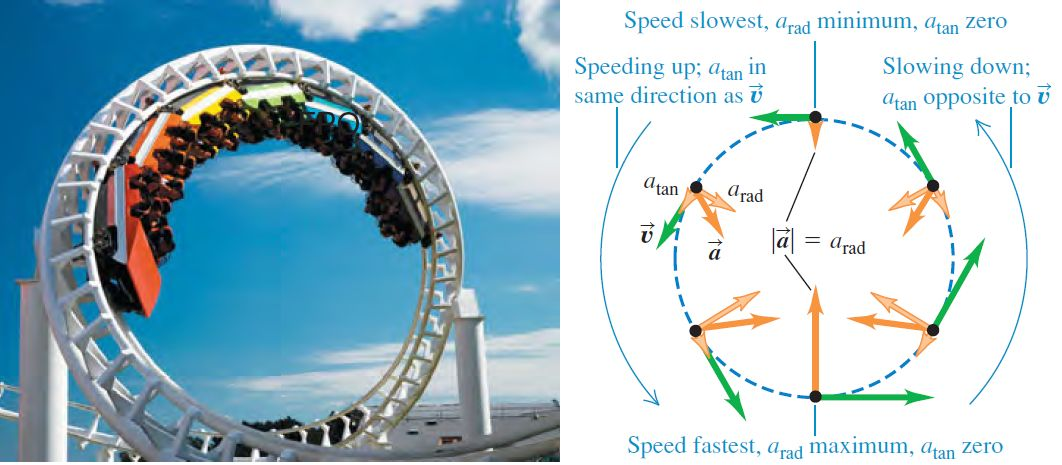
\includegraphics[width=1.\textwidth]{images/37.jpg}
      \caption{ {\tiny Figures from Sears and Zemansky's University Physics 
      with Modern Physics, 13th Edition.} }
    \end{figure}
  
  
  
  
      \end{frame}
  
   %%%%%%%%%%%%%%%%%%%%%%%%%%%%%%%%%%%%%%%%%%%%%%%%%%%%%%%%%%%%%%%%%%%

 \begin{frame}
    Nonuniform Circular Motion
    
    
    
 \begin{enumerate}
    \item The speed varies.
    \item the radial component of acceleration is $a_{rad}=\frac{v^2}{R}$.
    \item  $v$ changes $\rightarrow a$ changes.
    \item $\omega$ also changes.
    \item There is also a tangential component, $a_{tan}=\frac{d\vert \vec v \vert}{d t}$
 \end{enumerate}
    
    \vspace{5mm}
    \pause
    Let's define the angular acceleration:

    \begin{equation}
        \alpha=\frac{d \omega}{d t}
    \end{equation}

        \end{frame}
    
     %%%%%%%%%%%%%%%%%%%%%%%%%%%%%%%%%%%%%%%%%%%%%%%%%%%%%%%%%%%%%%%%%%%

      %%%%%%%%%%%%%%%%%%%%%%%%%%%%%%%%%%%%%%%%%%%%%%%%%%%%%%%%%%%%%%%%%%%


 \begin{frame}

    \begin{center}
        \begin{tabular}{| l |c |c |}
            \hline
         quantity & spacial & angular \\ 
         \hline
          &  &  \\ 
          coordinates & $x$ & $\theta$ \\  
          &  &  \\ 
         velocity & $v=\frac{d x}{d t}$ & $\omega=\frac{d \theta}{d t}$  \\
         &  &  \\ 
         acceleration & $a=\frac{d v}{d t}$ & $\alpha=\frac{d \omega}{d t}$  \\
         &  &  \\ 
         \hline
        \end{tabular}
        \end{center}


        Motion with constant angular accerelation:

        \begin{equation}
\theta(t)=\frac{1}{2}\alpha t^2+\omega_0 t+\theta_0
        \end{equation}


        \end{frame}
    
     %%%%%%%%%%%%%%%%%%%%%%%%%%%%%%%%%%%%%%%%%%%%%%%%%%%%%%%%%%%%%%%%%%%

        
    %%%%%%%%%%%%%%%%%%%%%%%%%%%%%%%%%%%%%%%%%%%%%%%%%%%%%%%%%%%%%%%%%%%

              
               %%%%%%%%%%%%%%%%%%%%%%%%%%%%%%%%%%%%%%%%%%%%%%%%%%%%%%%%%%%%%%%%%%%























%%%%%%%%%%%%%%%%%%%%%%%%%%%%%%%%%%%%%%%%%%%%%%%%%%%%%%%%%%%%%%%%%%%
 \end{document}
%%%%%%%%%%%%%%%%%%%%%%%%%%%%%%%%%%%%%%%%%%%%%%%%%%%%%%%%%%%%%%%%%%%